\chapter{Results}
\todo[inline]{some very nice graphs}

\section{Technical Details}
\begin{itemize}
  \item Intel\textsuperscript{\textregistered}~Core\texttrademark~2 Duo CPU E6850
  \item 2 GB RAM
  \item \todo[inline]{CGAL version}
\end{itemize}

\section{Segment Lengths}

\begin{figure}[ht]
  \centering
  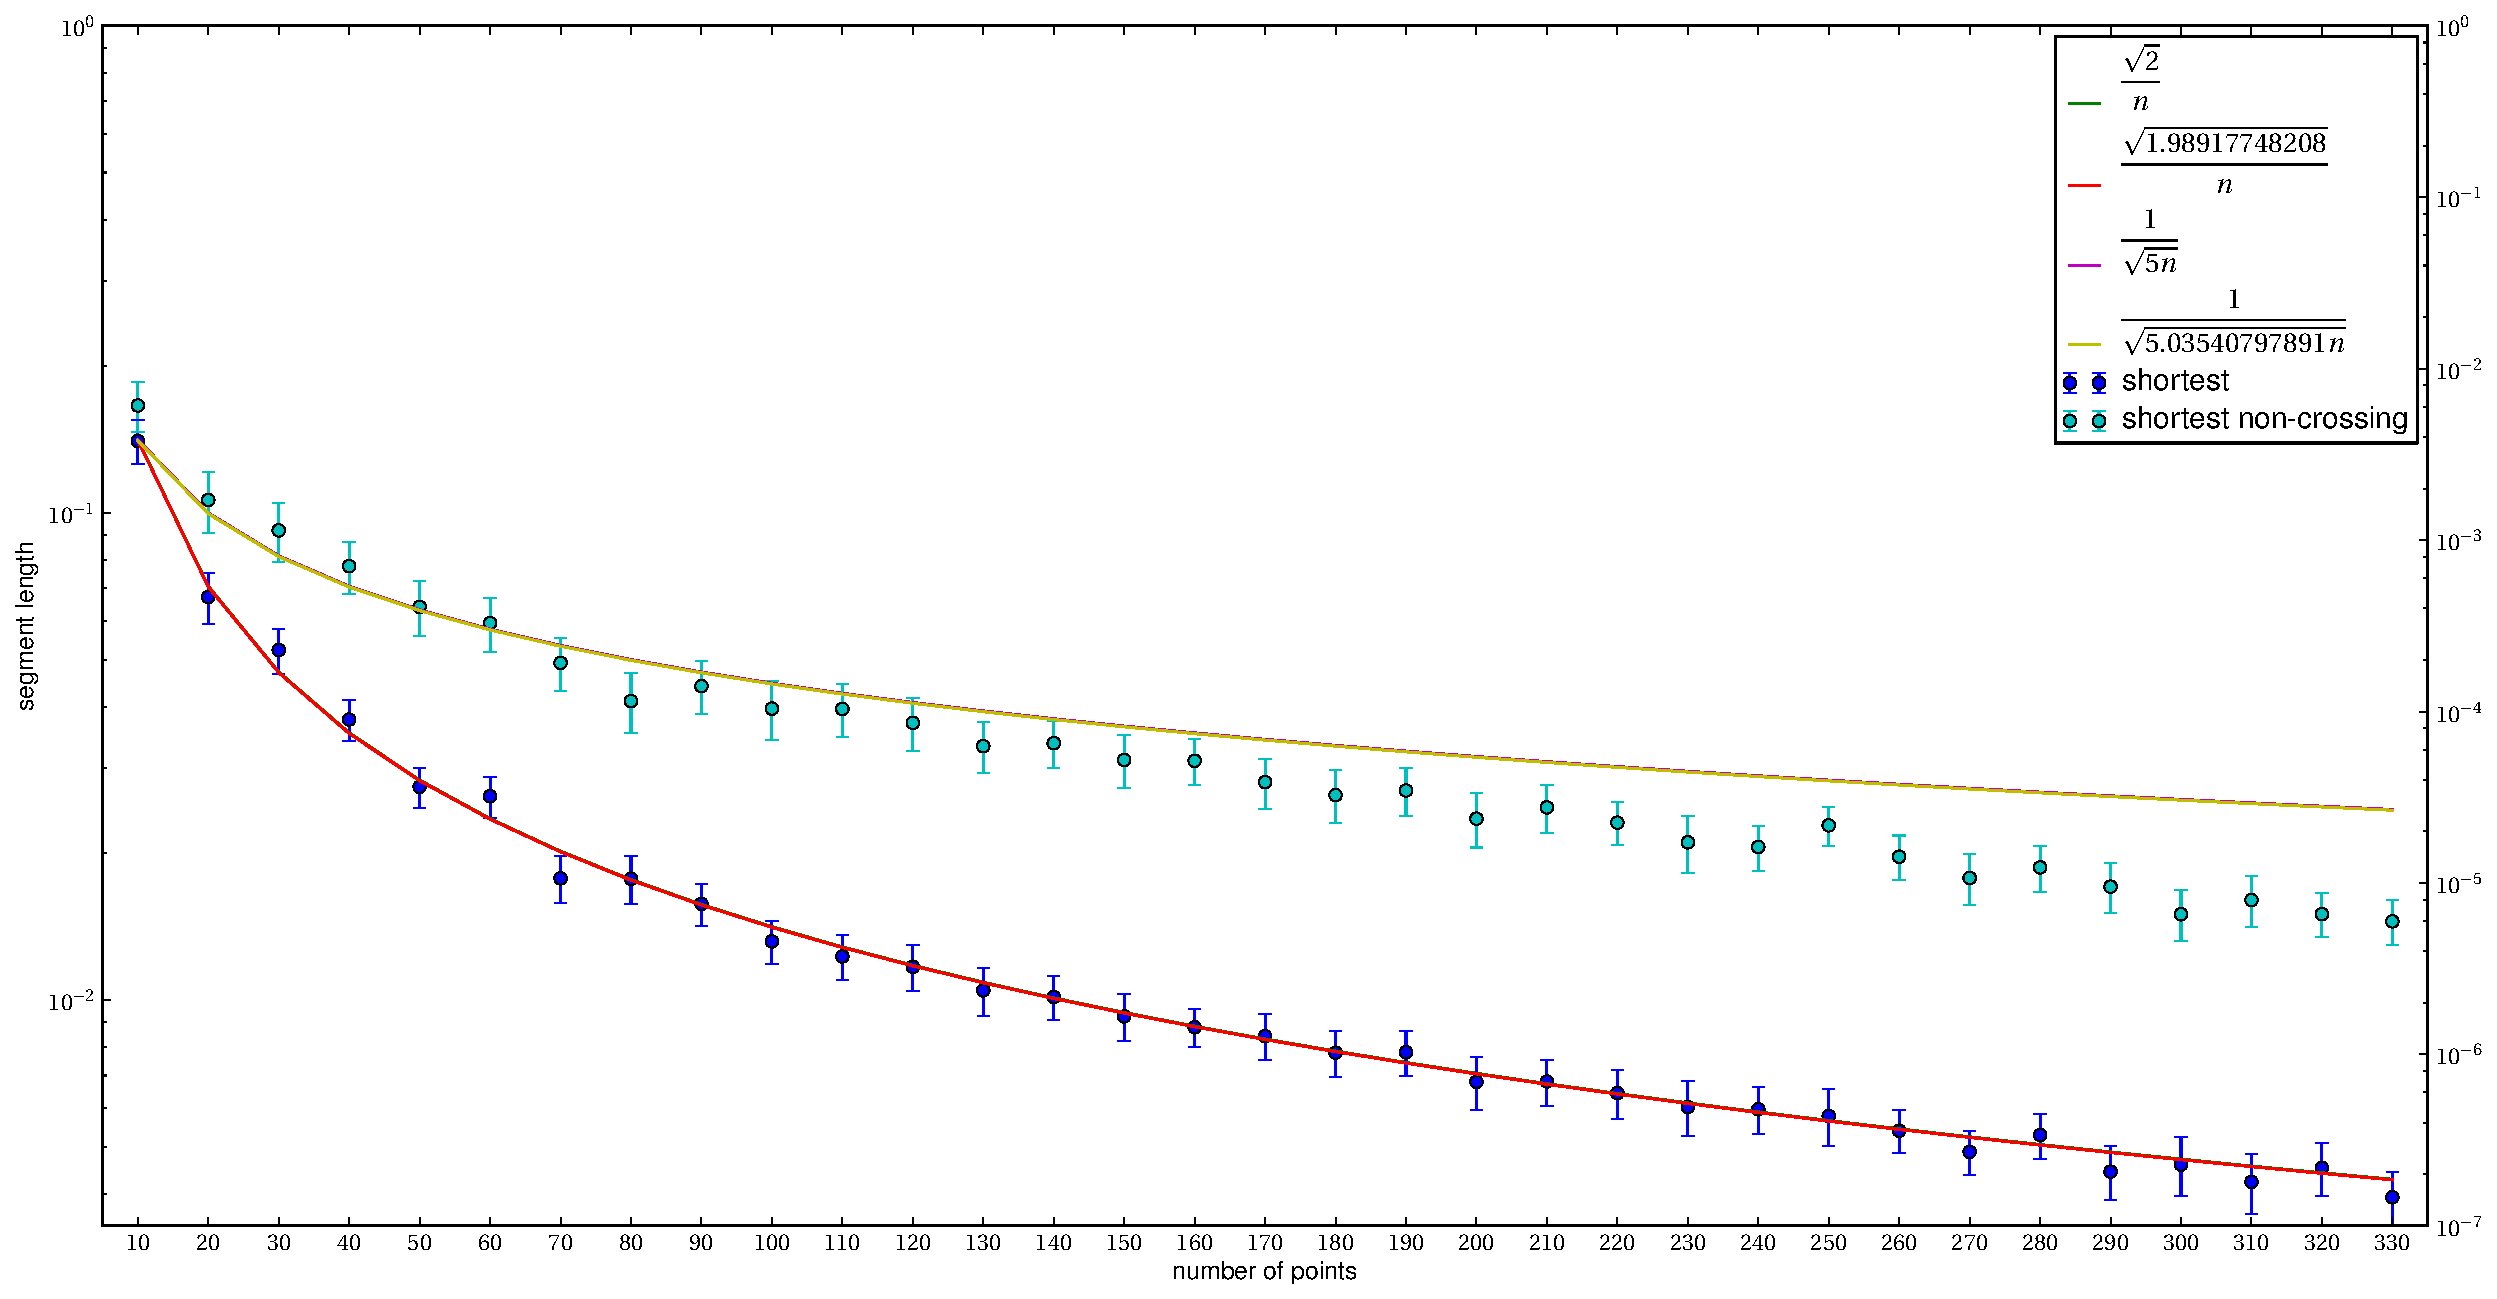
\includegraphics[width=0.9\textwidth]{results/shortest_length.pdf}
  \todo[inline]{replace}
  \caption{Comparison of segment lengths\label{fig:segment_lengths}}
\end{figure}

\begin{figure}[ht]
  \centering
  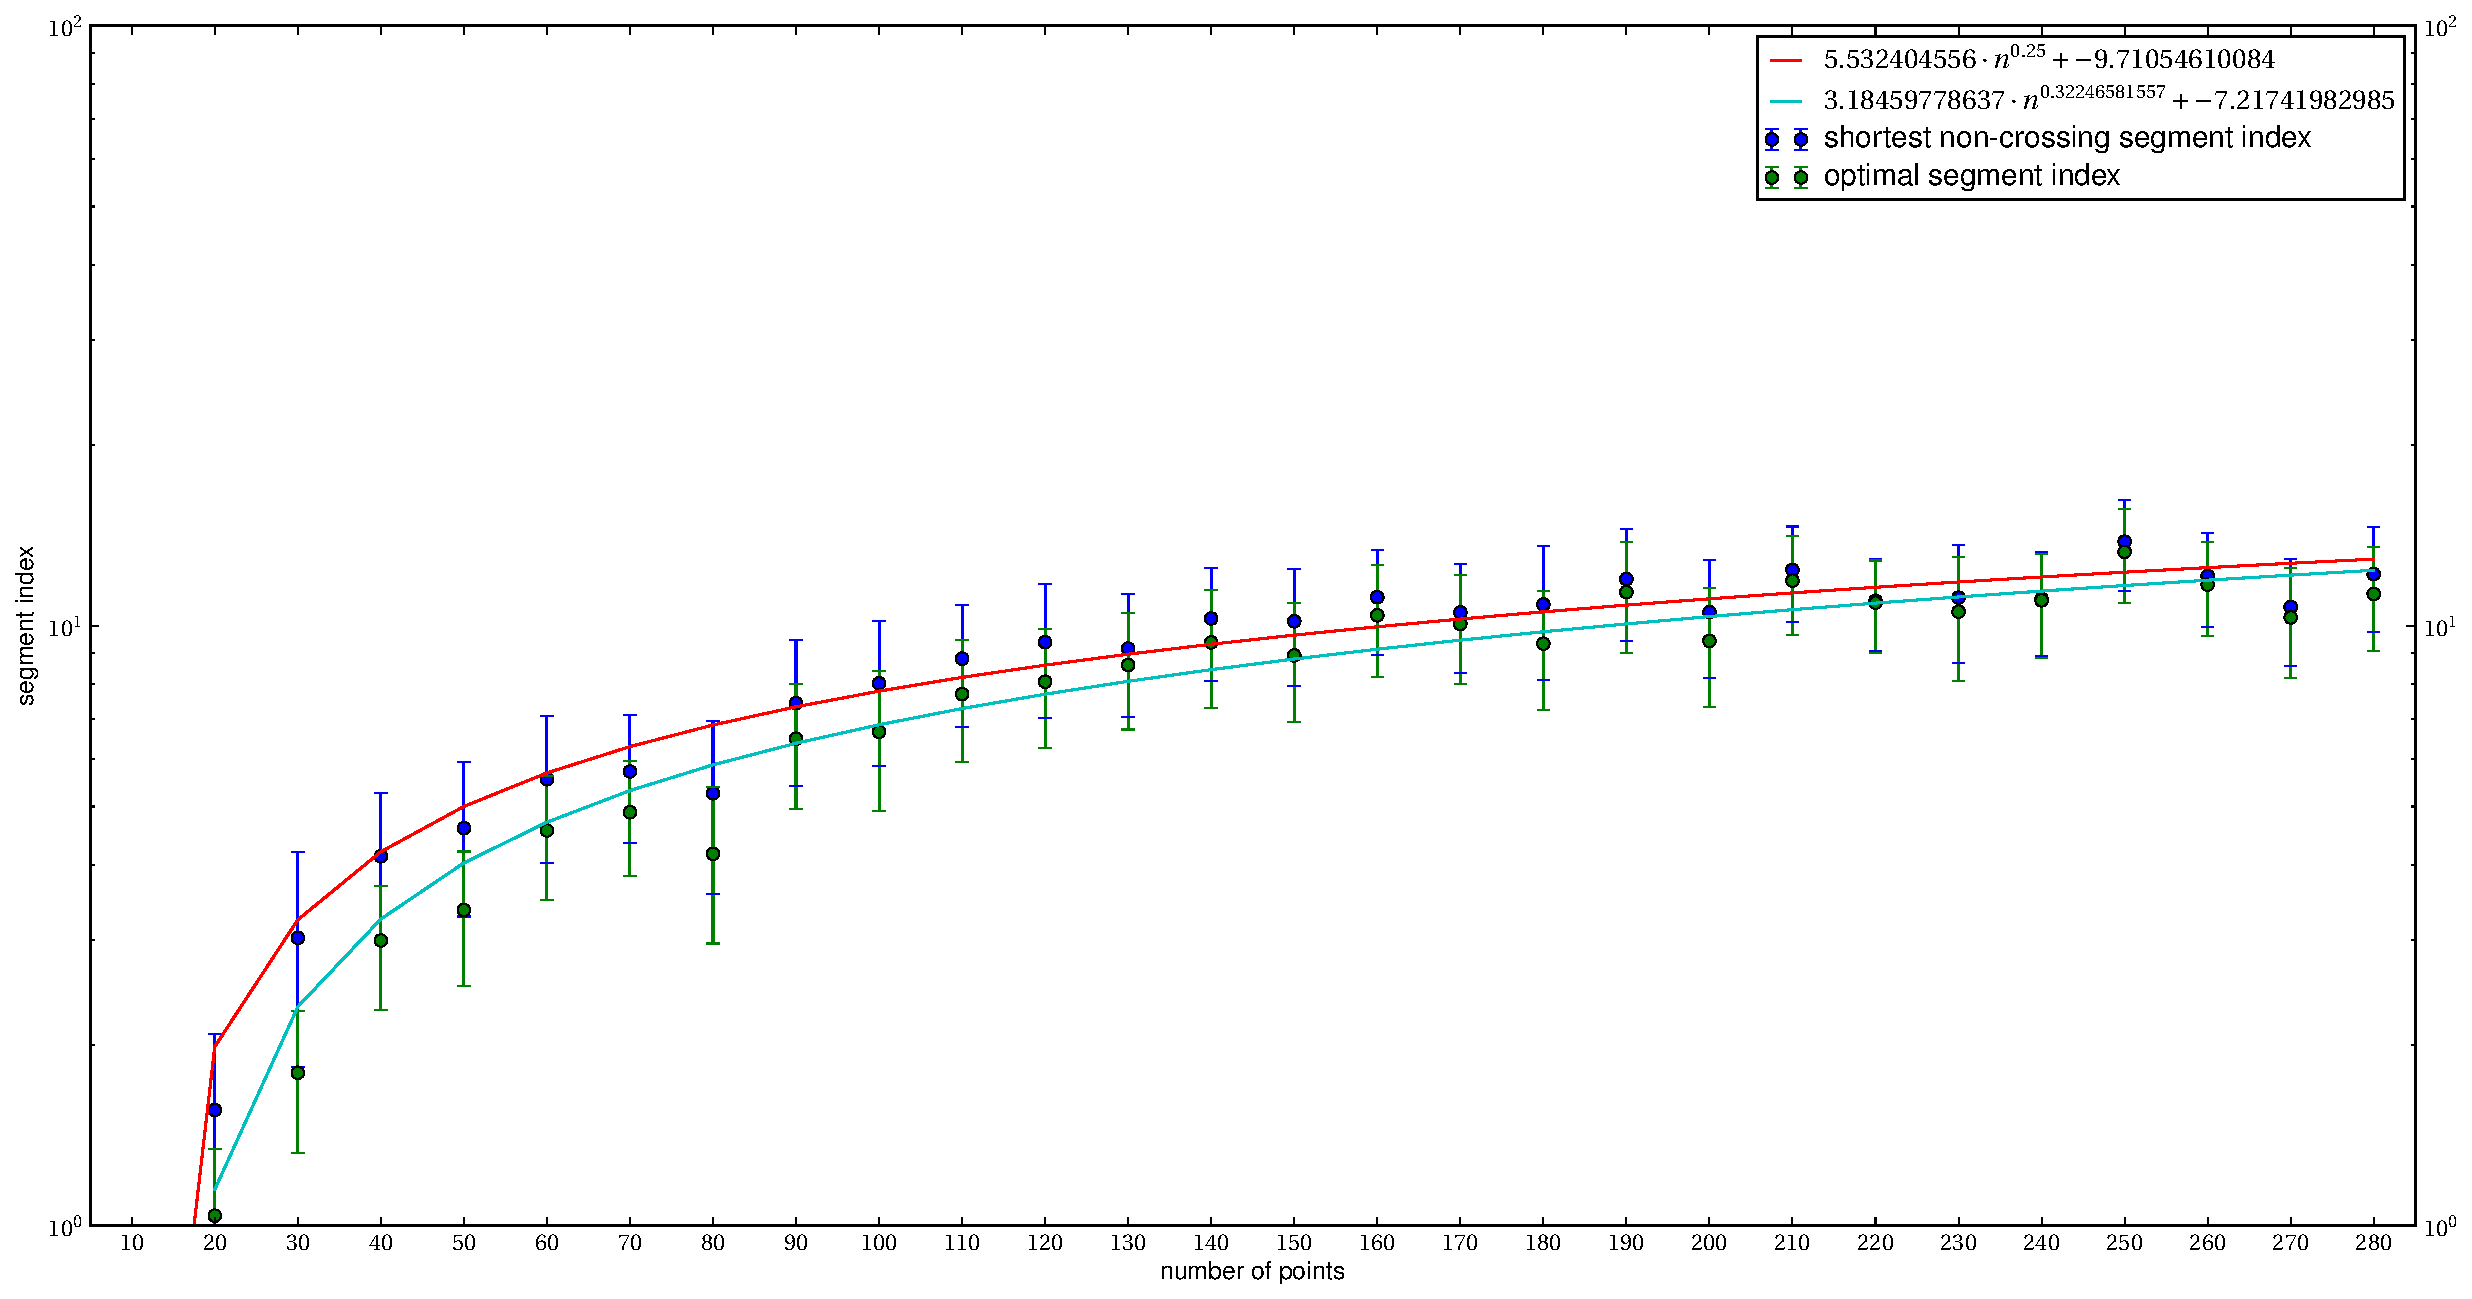
\includegraphics[width=0.9\textwidth]{results/shortest_index.pdf}
  \todo[inline]{replace}
  \caption{Comparison of segment indices\label{fig:segment_index}}
\end{figure}

\section{Execution Time}

\begin{figure}[ht]
  \centering
  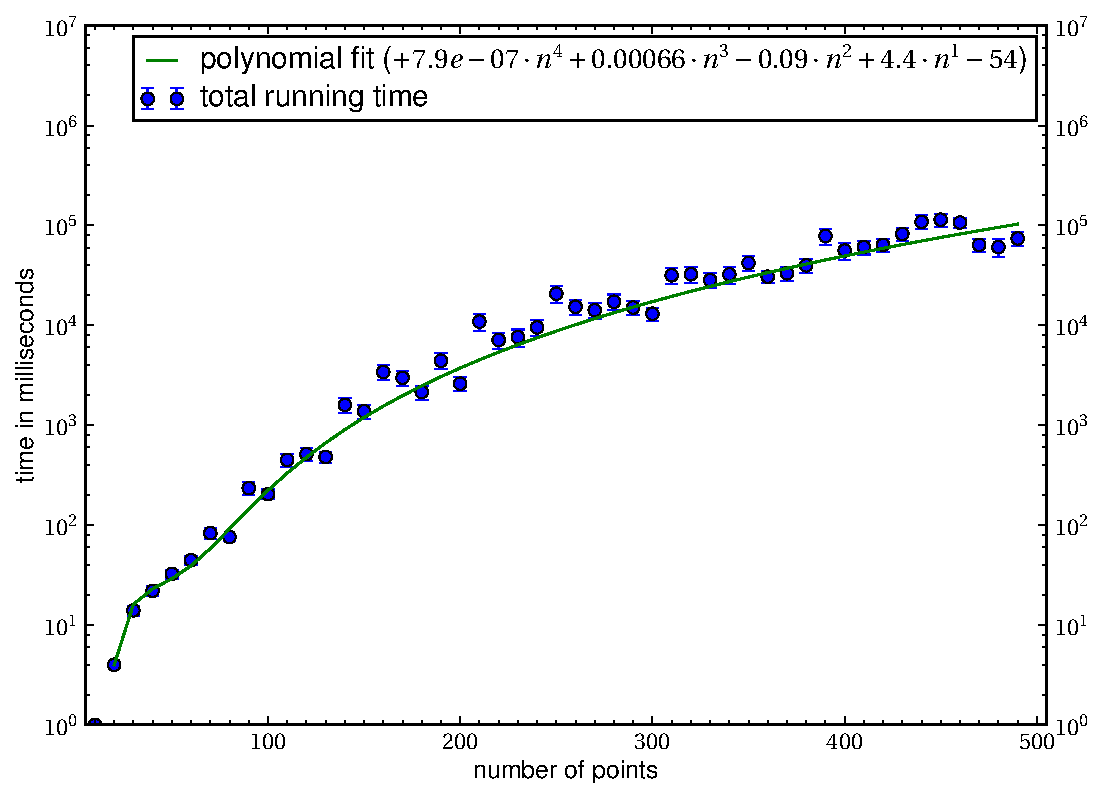
\includegraphics[width=0.9\textwidth]{results/time_total.pdf}
  \todo[inline]{replace}
  \caption{Total execution time\label{fig:total_time}}
\end{figure}

\begin{figure}[ht]
  \centering
  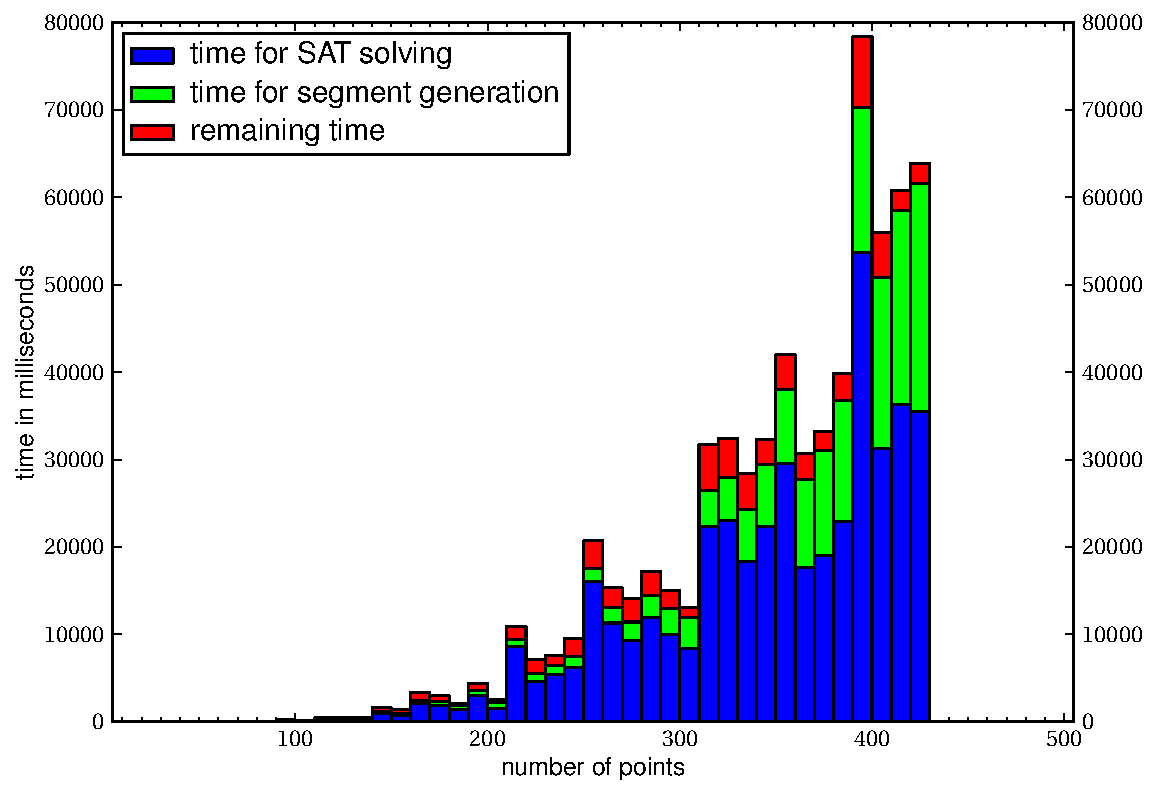
\includegraphics[width=0.9\textwidth]{results/time_comparison.pdf}
  \todo[inline]{replace}
  \caption{Comparison of execution times\label{fig:times}}
\end{figure}

\section{Aborted instances}

\begin{figure}[ht]
  \centering
  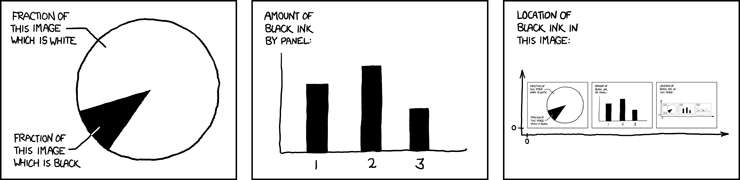
\includegraphics[width=0.5\textwidth]{img/self_description.png}
  \todo[inline]{replace}
  \caption{Number of aborted instances\label{fig:aborted}}
\end{figure}
